\documentclass[1p]{elsarticle_modified}
%\bibliographystyle{elsarticle-num}

%\usepackage[colorlinks]{hyperref}
%\usepackage{abbrmath_seonhwa} %\Abb, \Ascr, \Acal ,\Abf, \Afrak
\usepackage{amsfonts}
\usepackage{amssymb}
\usepackage{amsmath}
\usepackage{amsthm}
\usepackage{scalefnt}
\usepackage{amsbsy}
\usepackage{kotex}
\usepackage{caption}
\usepackage{subfig}
\usepackage{color}
\usepackage{graphicx}
\usepackage{xcolor} %% white, black, red, green, blue, cyan, magenta, yellow
\usepackage{float}
\usepackage{setspace}
\usepackage{hyperref}

\usepackage{tikz}
\usetikzlibrary{arrows}

\usepackage{multirow}
\usepackage{array} % fixed length table
\usepackage{hhline}

%%%%%%%%%%%%%%%%%%%%%
\makeatletter
\renewcommand*\env@matrix[1][\arraystretch]{%
	\edef\arraystretch{#1}%
	\hskip -\arraycolsep
	\let\@ifnextchar\new@ifnextchar
	\array{*\c@MaxMatrixCols c}}
\makeatother %https://tex.stackexchange.com/questions/14071/how-can-i-increase-the-line-spacing-in-a-matrix
%%%%%%%%%%%%%%%

\usepackage[normalem]{ulem}

\newcommand{\msout}[1]{\ifmmode\text{\sout{\ensuremath{#1}}}\else\sout{#1}\fi}
%SOURCE: \msout is \stkout macro in https://tex.stackexchange.com/questions/20609/strikeout-in-math-mode

\newcommand{\cancel}[1]{
	\ifmmode
	{\color{red}\msout{#1}}
	\else
	{\color{red}\sout{#1}}
	\fi
}

\newcommand{\add}[1]{
	{\color{blue}\uwave{#1}}
}

\newcommand{\replace}[2]{
	\ifmmode
	{\color{red}\msout{#1}}{\color{blue}\uwave{#2}}
	\else
	{\color{red}\sout{#1}}{\color{blue}\uwave{#2}}
	\fi
}

\newcommand{\Sol}{\mathcal{S}} %segment
\newcommand{\D}{D} %diagram
\newcommand{\A}{\mathcal{A}} %arc


%%%%%%%%%%%%%%%%%%%%%%%%%%%%%5 test

\def\sl{\operatorname{\textup{SL}}(2,\Cbb)}
\def\psl{\operatorname{\textup{PSL}}(2,\Cbb)}
\def\quan{\mkern 1mu \triangleright \mkern 1mu}

\theoremstyle{definition}
\newtheorem{thm}{Theorem}[section]
\newtheorem{prop}[thm]{Proposition}
\newtheorem{lem}[thm]{Lemma}
\newtheorem{ques}[thm]{Question}
\newtheorem{cor}[thm]{Corollary}
\newtheorem{defn}[thm]{Definition}
\newtheorem{exam}[thm]{Example}
\newtheorem{rmk}[thm]{Remark}
\newtheorem{alg}[thm]{Algorithm}

\newcommand{\I}{\sqrt{-1}}
\begin{document}

%\begin{frontmatter}
%
%\title{Boundary parabolic representations of knots up to 8 crossings}
%
%%% Group authors per affiliation:
%\author{Yunhi Cho} 
%\address{Department of Mathematics, University of Seoul, Seoul, Korea}
%\ead{yhcho@uos.ac.kr}
%
%
%\author{Seonhwa Kim} %\fnref{s_kim}}
%\address{Center for Geometry and Physics, Institute for Basic Science, Pohang, 37673, Korea}
%\ead{ryeona17@ibs.re.kr}
%
%\author{Hyuk Kim}
%\address{Department of Mathematical Sciences, Seoul National University, Seoul 08826, Korea}
%\ead{hyukkim@snu.ac.kr}
%
%\author{Seokbeom Yoon}
%\address{Department of Mathematical Sciences, Seoul National University, Seoul, 08826,  Korea}
%\ead{sbyoon15@snu.ac.kr}
%
%\begin{abstract}
%We find all boundary parabolic representation of knots up to 8 crossings.
%
%\end{abstract}
%\begin{keyword}
%    \MSC[2010] 57M25 
%\end{keyword}
%
%\end{frontmatter}

%\linenumbers
%\tableofcontents
%
\newcommand\colored[1]{\textcolor{white}{\rule[-0.35ex]{0.8em}{1.4ex}}\kern-0.8em\color{red} #1}%
%\newcommand\colored[1]{\textcolor{white}{ #1}\kern-2.17ex	\textcolor{white}{ #1}\kern-1.81ex	\textcolor{white}{ #1}\kern-2.15ex\color{red}#1	}

{\Large $\underline{12a_{0518}~(K12a_{0518})}$}

\setlength{\tabcolsep}{10pt}
\renewcommand{\arraystretch}{1.6}
\vspace{1cm}\begin{tabular}{m{100pt}>{\centering\arraybackslash}m{274pt}}
\multirow{5}{120pt}{
	\centering
	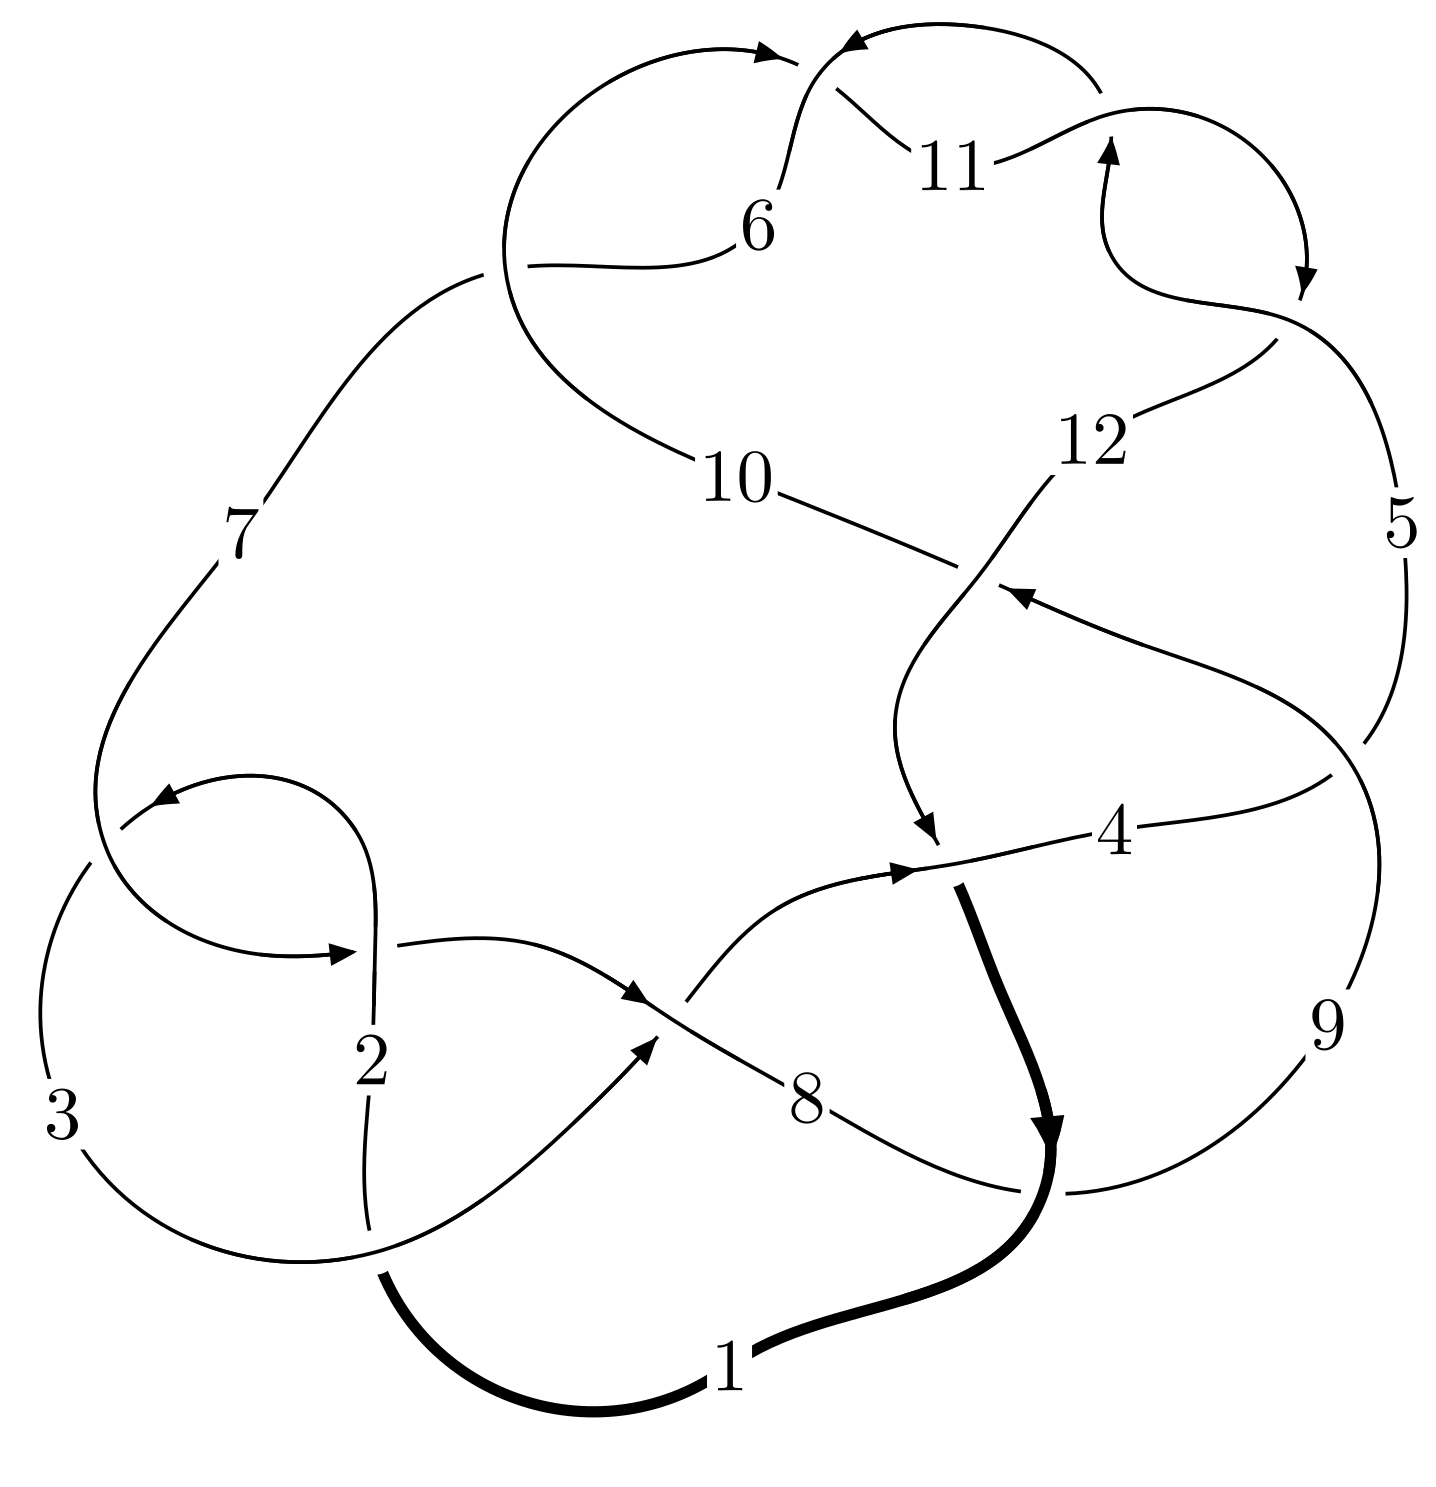
\includegraphics[width=112pt]{../../../GIT/diagram.site/Diagrams/png/1319_12a_0518.png}\\
\ \ \ A knot diagram\footnotemark}&
\allowdisplaybreaks
\textbf{Linearized knot diagam} \\
\cline{2-2}
 &
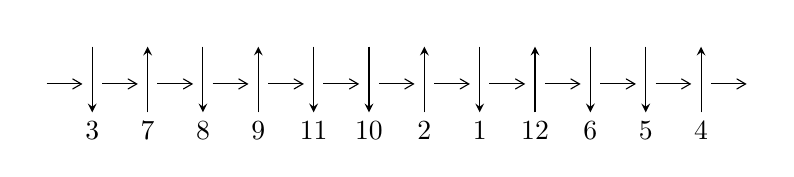
\begin{tikzpicture}[x=20pt, y=17pt]
	% nodes
	\node (C0) at (0, 0) {};
	\node (C1) at (1, 0) {};
	\node (C1U) at (1, +1) {};
	\node (C1D) at (1, -1) {3};

	\node (C2) at (2, 0) {};
	\node (C2U) at (2, +1) {};
	\node (C2D) at (2, -1) {7};

	\node (C3) at (3, 0) {};
	\node (C3U) at (3, +1) {};
	\node (C3D) at (3, -1) {8};

	\node (C4) at (4, 0) {};
	\node (C4U) at (4, +1) {};
	\node (C4D) at (4, -1) {9};

	\node (C5) at (5, 0) {};
	\node (C5U) at (5, +1) {};
	\node (C5D) at (5, -1) {11};

	\node (C6) at (6, 0) {};
	\node (C6U) at (6, +1) {};
	\node (C6D) at (6, -1) {10};

	\node (C7) at (7, 0) {};
	\node (C7U) at (7, +1) {};
	\node (C7D) at (7, -1) {2};

	\node (C8) at (8, 0) {};
	\node (C8U) at (8, +1) {};
	\node (C8D) at (8, -1) {1};

	\node (C9) at (9, 0) {};
	\node (C9U) at (9, +1) {};
	\node (C9D) at (9, -1) {12};

	\node (C10) at (10, 0) {};
	\node (C10U) at (10, +1) {};
	\node (C10D) at (10, -1) {6};

	\node (C11) at (11, 0) {};
	\node (C11U) at (11, +1) {};
	\node (C11D) at (11, -1) {5};

	\node (C12) at (12, 0) {};
	\node (C12U) at (12, +1) {};
	\node (C12D) at (12, -1) {4};
	\node (C13) at (13, 0) {};

	% arrows
	\draw[->,>={angle 60}]
	(C0) edge (C1) (C1) edge (C2) (C2) edge (C3) (C3) edge (C4) (C4) edge (C5) (C5) edge (C6) (C6) edge (C7) (C7) edge (C8) (C8) edge (C9) (C9) edge (C10) (C10) edge (C11) (C11) edge (C12) (C12) edge (C13) ;	\draw[->,>=stealth]
	(C1U) edge (C1D) (C2D) edge (C2U) (C3U) edge (C3D) (C4D) edge (C4U) (C5U) edge (C5D) (C6U) edge (C6D) (C7D) edge (C7U) (C8U) edge (C8D) (C9D) edge (C9U) (C10U) edge (C10D) (C11U) edge (C11D) (C12D) edge (C12U) ;
	\end{tikzpicture} \\
\hhline{~~} \\& 
\textbf{Solving Sequence} \\ \cline{2-2} 
 &
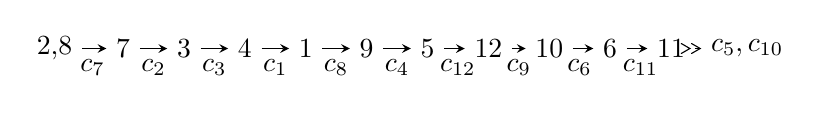
\begin{tikzpicture}[x=22pt, y=7pt]
	% node
	\node (A0) at (-1/8, 0) {2,8};
	\node (A1) at (1, 0) {7};
	\node (A2) at (2, 0) {3};
	\node (A3) at (3, 0) {4};
	\node (A4) at (4, 0) {1};
	\node (A5) at (5, 0) {9};
	\node (A6) at (6, 0) {5};
	\node (A7) at (7, 0) {12};
	\node (A8) at (8, 0) {10};
	\node (A9) at (9, 0) {6};
	\node (A10) at (10, 0) {11};
	\node (C1) at (1/2, -1) {$c_{7}$};
	\node (C2) at (3/2, -1) {$c_{2}$};
	\node (C3) at (5/2, -1) {$c_{3}$};
	\node (C4) at (7/2, -1) {$c_{1}$};
	\node (C5) at (9/2, -1) {$c_{8}$};
	\node (C6) at (11/2, -1) {$c_{4}$};
	\node (C7) at (13/2, -1) {$c_{12}$};
	\node (C8) at (15/2, -1) {$c_{9}$};
	\node (C9) at (17/2, -1) {$c_{6}$};
	\node (C10) at (19/2, -1) {$c_{11}$};
	\node (A11) at (45/4, 0) {$c_{5},c_{10}$};

	% edge
	\draw[->,>=stealth]	
	(A0) edge (A1) (A1) edge (A2) (A2) edge (A3) (A3) edge (A4) (A4) edge (A5) (A5) edge (A6) (A6) edge (A7) (A7) edge (A8) (A8) edge (A9) (A9) edge (A10) ;
	\draw[->>,>={angle 60}]	
	(A10) edge (A11);
\end{tikzpicture} \\ 

\end{tabular} \\

\footnotetext{
The image of knot diagram is generated by the software ``\textbf{Draw programme}" developed by Andrew Bartholomew(\url{http://www.layer8.co.uk/maths/draw/index.htm\#Running-draw}), where we modified some parts for our purpose(\url{https://github.com/CATsTAILs/LinksPainter}).
}\phantom \\ \newline 
\centering \textbf{Ideals for irreducible components\footnotemark of $X_{\text{par}}$} 
 
\begin{align*}
I^u_{1}&=\langle 
u^{78}+u^{77}+\cdots+u+1\rangle \\
\\
\end{align*}
\raggedright * 1 irreducible components of $\dim_{\mathbb{C}}=0$, with total 78 representations.\\
\footnotetext{All coefficients of polynomials are rational numbers. But the coefficients are sometimes approximated in decimal forms when there is not enough margin.}
\newpage
\renewcommand{\arraystretch}{1}
\centering \section*{I. $I^u_{1}= \langle u^{78}+u^{77}+\cdots+u+1 \rangle$}
\flushleft \textbf{(i) Arc colorings}\\
\begin{tabular}{m{7pt} m{180pt} m{7pt} m{180pt} }
\flushright $a_{2}=$&$\begin{pmatrix}0\\u\end{pmatrix}$ \\
\flushright $a_{8}=$&$\begin{pmatrix}1\\0\end{pmatrix}$ \\
\flushright $a_{7}=$&$\begin{pmatrix}1\\u^2\end{pmatrix}$ \\
\flushright $a_{3}=$&$\begin{pmatrix}u\\u^3+u\end{pmatrix}$ \\
\flushright $a_{4}=$&$\begin{pmatrix}- u^3\\u^3+u\end{pmatrix}$ \\
\flushright $a_{1}=$&$\begin{pmatrix}u^3\\u^5+u^3+u\end{pmatrix}$ \\
\flushright $a_{9}=$&$\begin{pmatrix}u^8+u^6+u^4+1\\u^{10}+2 u^8+3 u^6+2 u^4+u^2\end{pmatrix}$ \\
\flushright $a_{5}=$&$\begin{pmatrix}u^{21}+4 u^{19}+9 u^{17}+12 u^{15}+12 u^{13}+10 u^{11}+9 u^9+6 u^7+3 u^5+u\\u^{23}+5 u^{21}+\cdots+2 u^3+u\end{pmatrix}$ \\
\flushright $a_{12}=$&$\begin{pmatrix}- u^{11}-2 u^9-2 u^7+u^3\\u^{11}+3 u^9+4 u^7+3 u^5+u^3+u\end{pmatrix}$ \\
\flushright $a_{10}=$&$\begin{pmatrix}u^{32}+7 u^{30}+\cdots+2 u^{12}+1\\- u^{32}-8 u^{30}+\cdots-12 u^8-4 u^6\end{pmatrix}$ \\
\flushright $a_{6}=$&$\begin{pmatrix}u^{66}+15 u^{64}+\cdots+u^2+1\\- u^{66}-16 u^{64}+\cdots-4 u^8+u^2\end{pmatrix}$ \\
\flushright $a_{11}=$&$\begin{pmatrix}u^{55}+12 u^{53}+\cdots+5 u^7+2 u^3\\u^{57}+13 u^{55}+\cdots+2 u^3+u\end{pmatrix}$\\&\end{tabular}
\flushleft \textbf{(ii) Obstruction class $= -1$}\\~\\
\flushleft \textbf{(iii) Cusp Shapes $= -4 u^{76}-4 u^{75}+\cdots-8 u-6$}\\~\\
\newpage\renewcommand{\arraystretch}{1}
\flushleft \textbf{(iv) u-Polynomials at the component}\newline \\
\begin{tabular}{m{50pt}|m{274pt}}
Crossings & \hspace{64pt}u-Polynomials at each crossing \\
\hline $$\begin{aligned}c_{1}\end{aligned}$$&$\begin{aligned}
&u^{78}+37 u^{77}+\cdots+3 u+1
\end{aligned}$\\
\hline $$\begin{aligned}c_{2},c_{7}\end{aligned}$$&$\begin{aligned}
&u^{78}+u^{77}+\cdots+u+1
\end{aligned}$\\
\hline $$\begin{aligned}c_{3}\end{aligned}$$&$\begin{aligned}
&u^{78}- u^{77}+\cdots-711 u+185
\end{aligned}$\\
\hline $$\begin{aligned}c_{4}\end{aligned}$$&$\begin{aligned}
&u^{78}+u^{77}+\cdots-2625 u+2061
\end{aligned}$\\
\hline $$\begin{aligned}c_{5},c_{6},c_{10}\\c_{11}\end{aligned}$$&$\begin{aligned}
&u^{78}+u^{77}+\cdots+3 u+1
\end{aligned}$\\
\hline $$\begin{aligned}c_{8}\end{aligned}$$&$\begin{aligned}
&u^{78}+5 u^{77}+\cdots+233 u+259
\end{aligned}$\\
\hline $$\begin{aligned}c_{9}\end{aligned}$$&$\begin{aligned}
&u^{78}+21 u^{77}+\cdots+3489 u+187
\end{aligned}$\\
\hline $$\begin{aligned}c_{12}\end{aligned}$$&$\begin{aligned}
&u^{78}+9 u^{77}+\cdots+1209 u+109
\end{aligned}$\\
\hline
\end{tabular}\\~\\
\newpage\renewcommand{\arraystretch}{1}
\flushleft \textbf{(v) Riley Polynomials at the component}\newline \\
\begin{tabular}{m{50pt}|m{274pt}}
Crossings & \hspace{64pt}Riley Polynomials at each crossing \\
\hline $$\begin{aligned}c_{1}\end{aligned}$$&$\begin{aligned}
&y^{78}+9 y^{77}+\cdots+7 y+1
\end{aligned}$\\
\hline $$\begin{aligned}c_{2},c_{7}\end{aligned}$$&$\begin{aligned}
&y^{78}+37 y^{77}+\cdots+3 y+1
\end{aligned}$\\
\hline $$\begin{aligned}c_{3}\end{aligned}$$&$\begin{aligned}
&y^{78}-19 y^{77}+\cdots-1149321 y+34225
\end{aligned}$\\
\hline $$\begin{aligned}c_{4}\end{aligned}$$&$\begin{aligned}
&y^{78}-27 y^{77}+\cdots-82982745 y+4247721
\end{aligned}$\\
\hline $$\begin{aligned}c_{5},c_{6},c_{10}\\c_{11}\end{aligned}$$&$\begin{aligned}
&y^{78}+89 y^{77}+\cdots+3 y+1
\end{aligned}$\\
\hline $$\begin{aligned}c_{8}\end{aligned}$$&$\begin{aligned}
&y^{78}+17 y^{77}+\cdots+3777875 y+67081
\end{aligned}$\\
\hline $$\begin{aligned}c_{9}\end{aligned}$$&$\begin{aligned}
&y^{78}-11 y^{77}+\cdots-42057 y+34969
\end{aligned}$\\
\hline $$\begin{aligned}c_{12}\end{aligned}$$&$\begin{aligned}
&y^{78}+13 y^{77}+\cdots+852607 y+11881
\end{aligned}$\\
\hline
\end{tabular}\\~\\
\newpage\flushleft \textbf{(vi) Complex Volumes and Cusp Shapes}
$$\begin{array}{c|c|c}  
\text{Solutions to }I^u_{1}& \I (\text{vol} + \sqrt{-1}CS) & \text{Cusp shape}\\
 \hline 
\begin{aligned}
u &= -0.176293 + 1.038900 I\end{aligned}
 & \phantom{-}7.18444 - 1.67019 I & \phantom{-0.000000 } 0 \\ \hline\begin{aligned}
u &= -0.176293 - 1.038900 I\end{aligned}
 & \phantom{-}7.18444 + 1.67019 I & \phantom{-0.000000 } 0 \\ \hline\begin{aligned}
u &= \phantom{-}0.250777 + 1.048820 I\end{aligned}
 & -0.743942 + 0.717138 I & \phantom{-0.000000 } 0 \\ \hline\begin{aligned}
u &= \phantom{-}0.250777 - 1.048820 I\end{aligned}
 & -0.743942 - 0.717138 I & \phantom{-0.000000 } 0 \\ \hline\begin{aligned}
u &= \phantom{-}0.662622 + 0.622414 I\end{aligned}
 & \phantom{-}11.08790 + 7.77112 I & \phantom{-}6.08947 - 6.15924 I \\ \hline\begin{aligned}
u &= \phantom{-}0.662622 - 0.622414 I\end{aligned}
 & \phantom{-}11.08790 - 7.77112 I & \phantom{-}6.08947 + 6.15924 I \\ \hline\begin{aligned}
u &= -0.559696 + 0.953541 I\end{aligned}
 & \phantom{-}2.23246 + 0.83804 I & \phantom{-0.000000 } 0 \\ \hline\begin{aligned}
u &= -0.559696 - 0.953541 I\end{aligned}
 & \phantom{-}2.23246 - 0.83804 I & \phantom{-0.000000 } 0 \\ \hline\begin{aligned}
u &= -0.644680 + 0.615060 I\end{aligned}
 & \phantom{-}3.22743 - 5.55791 I & \phantom{-}3.92619 + 8.07198 I \\ \hline\begin{aligned}
u &= -0.644680 - 0.615060 I\end{aligned}
 & \phantom{-}3.22743 + 5.55791 I & \phantom{-}3.92619 - 8.07198 I \\ \hline\begin{aligned}
u &= \phantom{-}0.578452 + 0.948103 I\end{aligned}
 & \phantom{-}10.12780 - 2.94206 I & \phantom{-0.000000 } 0 \\ \hline\begin{aligned}
u &= \phantom{-}0.578452 - 0.948103 I\end{aligned}
 & \phantom{-}10.12780 + 2.94206 I & \phantom{-0.000000 } 0 \\ \hline\begin{aligned}
u &= \phantom{-}0.536776 + 0.978594 I\end{aligned}
 & \phantom{-}0.45641 + 2.41567 I & \phantom{-0.000000 } 0 \\ \hline\begin{aligned}
u &= \phantom{-}0.536776 - 0.978594 I\end{aligned}
 & \phantom{-}0.45641 - 2.41567 I & \phantom{-0.000000 } 0 \\ \hline\begin{aligned}
u &= -0.494251 + 0.718740 I\end{aligned}
 & \phantom{-}6.27468 - 2.02964 I & \phantom{-}2.37275 + 3.90100 I \\ \hline\begin{aligned}
u &= -0.494251 - 0.718740 I\end{aligned}
 & \phantom{-}6.27468 + 2.02964 I & \phantom{-}2.37275 - 3.90100 I \\ \hline\begin{aligned}
u &= \phantom{-}0.679159 + 0.543155 I\end{aligned}
 & \phantom{-}12.45010 - 1.87294 I & \phantom{-}7.91266 + 0.01624 I \\ \hline\begin{aligned}
u &= \phantom{-}0.679159 - 0.543155 I\end{aligned}
 & \phantom{-}12.45010 + 1.87294 I & \phantom{-}7.91266 - 0.01624 I \\ \hline\begin{aligned}
u &= -0.248111 + 1.111540 I\end{aligned}
 & -4.03405 + 1.38195 I & \phantom{-0.000000 } 0 \\ \hline\begin{aligned}
u &= -0.248111 - 1.111540 I\end{aligned}
 & -4.03405 - 1.38195 I & \phantom{-0.000000 } 0 \\ \hline\begin{aligned}
u &= \phantom{-}0.617031 + 0.594101 I\end{aligned}
 & \phantom{-}1.58657 + 2.14626 I & \phantom{-}0.09014 - 3.07268 I \\ \hline\begin{aligned}
u &= \phantom{-}0.617031 - 0.594101 I\end{aligned}
 & \phantom{-}1.58657 - 2.14626 I & \phantom{-}0.09014 + 3.07268 I \\ \hline\begin{aligned}
u &= \phantom{-}0.231696 + 1.122790 I\end{aligned}
 & -2.66484 - 4.98283 I & \phantom{-0.000000 } 0 \\ \hline\begin{aligned}
u &= \phantom{-}0.231696 - 1.122790 I\end{aligned}
 & -2.66484 + 4.98283 I & \phantom{-0.000000 } 0 \\ \hline\begin{aligned}
u &= -0.220916 + 1.130910 I\end{aligned}
 & \phantom{-}5.04714 + 7.32940 I & \phantom{-0.000000 } 0 \\ \hline\begin{aligned}
u &= -0.220916 - 1.130910 I\end{aligned}
 & \phantom{-}5.04714 - 7.32940 I & \phantom{-0.000000 } 0 \\ \hline\begin{aligned}
u &= -0.561401 + 1.006840 I\end{aligned}
 & \phantom{-}2.94053 - 5.15801 I & \phantom{-0.000000 } 0 \\ \hline\begin{aligned}
u &= -0.561401 - 1.006840 I\end{aligned}
 & \phantom{-}2.94053 + 5.15801 I & \phantom{-0.000000 } 0 \\ \hline\begin{aligned}
u &= -0.646275 + 0.544185 I\end{aligned}
 & \phantom{-}4.30217 + 0.43226 I & \phantom{-}6.84123 - 1.12347 I \\ \hline\begin{aligned}
u &= -0.646275 - 0.544185 I\end{aligned}
 & \phantom{-}4.30217 - 0.43226 I & \phantom{-}6.84123 + 1.12347 I\\
 \hline 
 \end{array}$$\newpage$$\begin{array}{c|c|c}  
\text{Solutions to }I^u_{1}& \I (\text{vol} + \sqrt{-1}CS) & \text{Cusp shape}\\
 \hline 
\begin{aligned}
u &= -0.769714 + 0.344540 I\end{aligned}
 & \phantom{-}9.68605 + 10.02470 I & \phantom{-}4.54215 - 5.70117 I \\ \hline\begin{aligned}
u &= -0.769714 - 0.344540 I\end{aligned}
 & \phantom{-}9.68605 - 10.02470 I & \phantom{-}4.54215 + 5.70117 I \\ \hline\begin{aligned}
u &= -0.330134 + 1.108880 I\end{aligned}
 & -4.86646 - 1.53988 I & \phantom{-0.000000 } 0 \\ \hline\begin{aligned}
u &= -0.330134 - 1.108880 I\end{aligned}
 & -4.86646 + 1.53988 I & \phantom{-0.000000 } 0 \\ \hline\begin{aligned}
u &= \phantom{-}0.294729 + 1.123740 I\end{aligned}
 & \phantom{-}0.529229 - 0.096011 I & \phantom{-0.000000 } 0 \\ \hline\begin{aligned}
u &= \phantom{-}0.294729 - 1.123740 I\end{aligned}
 & \phantom{-}0.529229 + 0.096011 I & \phantom{-0.000000 } 0 \\ \hline\begin{aligned}
u &= -0.734635 + 0.397114 I\end{aligned}
 & \phantom{-}11.73850 + 0.41110 I & \phantom{-}7.04886 - 0.50949 I \\ \hline\begin{aligned}
u &= -0.734635 - 0.397114 I\end{aligned}
 & \phantom{-}11.73850 - 0.41110 I & \phantom{-}7.04886 + 0.50949 I \\ \hline\begin{aligned}
u &= \phantom{-}0.580481 + 1.010610 I\end{aligned}
 & \phantom{-}11.07250 + 6.74859 I & \phantom{-0.000000 } 0 \\ \hline\begin{aligned}
u &= \phantom{-}0.580481 - 1.010610 I\end{aligned}
 & \phantom{-}11.07250 - 6.74859 I & \phantom{-0.000000 } 0 \\ \hline\begin{aligned}
u &= \phantom{-}0.758266 + 0.340646 I\end{aligned}
 & \phantom{-}1.87500 - 7.66822 I & \phantom{-}2.06566 + 7.50138 I \\ \hline\begin{aligned}
u &= \phantom{-}0.758266 - 0.340646 I\end{aligned}
 & \phantom{-}1.87500 + 7.66822 I & \phantom{-}2.06566 - 7.50138 I \\ \hline\begin{aligned}
u &= \phantom{-}0.353897 + 1.116280 I\end{aligned}
 & -3.95417 + 5.01127 I & \phantom{-0.000000 } 0 \\ \hline\begin{aligned}
u &= \phantom{-}0.353897 - 1.116280 I\end{aligned}
 & -3.95417 - 5.01127 I & \phantom{-0.000000 } 0 \\ \hline\begin{aligned}
u &= -0.369372 + 1.126780 I\end{aligned}
 & \phantom{-}3.43300 - 7.21980 I & \phantom{-0.000000 } 0 \\ \hline\begin{aligned}
u &= -0.369372 - 1.126780 I\end{aligned}
 & \phantom{-}3.43300 + 7.21980 I & \phantom{-0.000000 } 0 \\ \hline\begin{aligned}
u &= -0.739839 + 0.336830 I\end{aligned}
 & \phantom{-}0.35594 + 4.04760 I & -1.60822 - 2.48146 I \\ \hline\begin{aligned}
u &= -0.739839 - 0.336830 I\end{aligned}
 & \phantom{-}0.35594 - 4.04760 I & -1.60822 + 2.48146 I \\ \hline\begin{aligned}
u &= \phantom{-}0.716830 + 0.371362 I\end{aligned}
 & \phantom{-}3.50311 - 1.57237 I & \phantom{-}5.70399 - 0.07635 I \\ \hline\begin{aligned}
u &= \phantom{-}0.716830 - 0.371362 I\end{aligned}
 & \phantom{-}3.50311 + 1.57237 I & \phantom{-}5.70399 + 0.07635 I \\ \hline\begin{aligned}
u &= -0.481533 + 1.115440 I\end{aligned}
 & \phantom{-}4.18249 - 0.46735 I & \phantom{-0.000000 } 0 \\ \hline\begin{aligned}
u &= -0.481533 - 1.115440 I\end{aligned}
 & \phantom{-}4.18249 + 0.46735 I & \phantom{-0.000000 } 0 \\ \hline\begin{aligned}
u &= \phantom{-}0.501259 + 1.108890 I\end{aligned}
 & -2.96742 + 2.54824 I & \phantom{-0.000000 } 0 \\ \hline\begin{aligned}
u &= \phantom{-}0.501259 - 1.108890 I\end{aligned}
 & -2.96742 - 2.54824 I & \phantom{-0.000000 } 0 \\ \hline\begin{aligned}
u &= -0.520445 + 1.111910 I\end{aligned}
 & -3.57499 - 5.99088 I & \phantom{-0.000000 } 0 \\ \hline\begin{aligned}
u &= -0.520445 - 1.111910 I\end{aligned}
 & -3.57499 + 5.99088 I & \phantom{-0.000000 } 0 \\ \hline\begin{aligned}
u &= \phantom{-}0.562822 + 1.102750 I\end{aligned}
 & \phantom{-}1.36314 + 6.46891 I & \phantom{-0.000000 } 0 \\ \hline\begin{aligned}
u &= \phantom{-}0.562822 - 1.102750 I\end{aligned}
 & \phantom{-}1.36314 - 6.46891 I & \phantom{-0.000000 } 0 \\ \hline\begin{aligned}
u &= -0.575491 + 1.096660 I\end{aligned}
 & \phantom{-}9.68171 - 5.40055 I & \phantom{-0.000000 } 0 \\ \hline\begin{aligned}
u &= -0.575491 - 1.096660 I\end{aligned}
 & \phantom{-}9.68171 + 5.40055 I & \phantom{-0.000000 } 0\\
 \hline 
 \end{array}$$\newpage$$\begin{array}{c|c|c}  
\text{Solutions to }I^u_{1}& \I (\text{vol} + \sqrt{-1}CS) & \text{Cusp shape}\\
 \hline 
\begin{aligned}
u &= \phantom{-}0.708462 + 0.274901 I\end{aligned}
 & \phantom{-}4.60181 - 3.06647 I & \phantom{-}0.82477 + 2.99322 I \\ \hline\begin{aligned}
u &= \phantom{-}0.708462 - 0.274901 I\end{aligned}
 & \phantom{-}4.60181 + 3.06647 I & \phantom{-}0.82477 - 2.99322 I \\ \hline\begin{aligned}
u &= \phantom{-}0.537436 + 1.123660 I\end{aligned}
 & \phantom{-}2.16314 + 7.81098 I & \phantom{-0.000000 } 0 \\ \hline\begin{aligned}
u &= \phantom{-}0.537436 - 1.123660 I\end{aligned}
 & \phantom{-}2.16314 - 7.81098 I & \phantom{-0.000000 } 0 \\ \hline\begin{aligned}
u &= -0.562734 + 1.119050 I\end{aligned}
 & -1.93087 - 8.99165 I & \phantom{-0.000000 } 0 \\ \hline\begin{aligned}
u &= -0.562734 - 1.119050 I\end{aligned}
 & -1.93087 + 8.99165 I & \phantom{-0.000000 } 0 \\ \hline\begin{aligned}
u &= \phantom{-}0.569133 + 1.122950 I\end{aligned}
 & -0.42249 + 12.68200 I & \phantom{-0.000000 } 0 \\ \hline\begin{aligned}
u &= \phantom{-}0.569133 - 1.122950 I\end{aligned}
 & -0.42249 - 12.68200 I & \phantom{-0.000000 } 0 \\ \hline\begin{aligned}
u &= -0.573825 + 1.125130 I\end{aligned}
 & \phantom{-}7.3870 - 15.0855 I & \phantom{-0.000000 } 0 \\ \hline\begin{aligned}
u &= -0.573825 - 1.125130 I\end{aligned}
 & \phantom{-}7.3870 + 15.0855 I & \phantom{-0.000000 } 0 \\ \hline\begin{aligned}
u &= -0.642804 + 0.250728 I\end{aligned}
 & -1.16696 + 1.46809 I & -3.90843 - 3.90329 I \\ \hline\begin{aligned}
u &= -0.642804 - 0.250728 I\end{aligned}
 & -1.16696 - 1.46809 I & -3.90843 + 3.90329 I \\ \hline\begin{aligned}
u &= \phantom{-}0.243242 + 0.611279 I\end{aligned}
 & -0.183340 + 1.154680 I & -2.33672 - 6.24031 I \\ \hline\begin{aligned}
u &= \phantom{-}0.243242 - 0.611279 I\end{aligned}
 & -0.183340 - 1.154680 I & -2.33672 + 6.24031 I \\ \hline\begin{aligned}
u &= -0.645299 + 0.117141 I\end{aligned}
 & \phantom{-}6.90376 - 3.74824 I & \phantom{-}1.81576 + 2.40321 I \\ \hline\begin{aligned}
u &= -0.645299 - 0.117141 I\end{aligned}
 & \phantom{-}6.90376 + 3.74824 I & \phantom{-}1.81576 - 2.40321 I \\ \hline\begin{aligned}
u &= \phantom{-}0.614376 + 0.171121 I\end{aligned}
 & -0.44935 + 1.76162 I & -1.34285 - 4.29386 I \\ \hline\begin{aligned}
u &= \phantom{-}0.614376 - 0.171121 I\end{aligned}
 & -0.44935 - 1.76162 I & -1.34285 + 4.29386 I\\
 \hline 
 \end{array}$$\newpage
\newpage\renewcommand{\arraystretch}{1}
\centering \section*{ II. u-Polynomials}
\begin{tabular}{m{50pt}|m{274pt}}
Crossings & \hspace{64pt}u-Polynomials at each crossing \\
\hline $$\begin{aligned}c_{1}\end{aligned}$$&$\begin{aligned}
&u^{78}+37 u^{77}+\cdots+3 u+1
\end{aligned}$\\
\hline $$\begin{aligned}c_{2},c_{7}\end{aligned}$$&$\begin{aligned}
&u^{78}+u^{77}+\cdots+u+1
\end{aligned}$\\
\hline $$\begin{aligned}c_{3}\end{aligned}$$&$\begin{aligned}
&u^{78}- u^{77}+\cdots-711 u+185
\end{aligned}$\\
\hline $$\begin{aligned}c_{4}\end{aligned}$$&$\begin{aligned}
&u^{78}+u^{77}+\cdots-2625 u+2061
\end{aligned}$\\
\hline $$\begin{aligned}c_{5},c_{6},c_{10}\\c_{11}\end{aligned}$$&$\begin{aligned}
&u^{78}+u^{77}+\cdots+3 u+1
\end{aligned}$\\
\hline $$\begin{aligned}c_{8}\end{aligned}$$&$\begin{aligned}
&u^{78}+5 u^{77}+\cdots+233 u+259
\end{aligned}$\\
\hline $$\begin{aligned}c_{9}\end{aligned}$$&$\begin{aligned}
&u^{78}+21 u^{77}+\cdots+3489 u+187
\end{aligned}$\\
\hline $$\begin{aligned}c_{12}\end{aligned}$$&$\begin{aligned}
&u^{78}+9 u^{77}+\cdots+1209 u+109
\end{aligned}$\\
\hline
\end{tabular}\newpage\renewcommand{\arraystretch}{1}
\centering \section*{ III. Riley Polynomials}
\begin{tabular}{m{50pt}|m{274pt}}
Crossings & \hspace{64pt}Riley Polynomials at each crossing \\
\hline $$\begin{aligned}c_{1}\end{aligned}$$&$\begin{aligned}
&y^{78}+9 y^{77}+\cdots+7 y+1
\end{aligned}$\\
\hline $$\begin{aligned}c_{2},c_{7}\end{aligned}$$&$\begin{aligned}
&y^{78}+37 y^{77}+\cdots+3 y+1
\end{aligned}$\\
\hline $$\begin{aligned}c_{3}\end{aligned}$$&$\begin{aligned}
&y^{78}-19 y^{77}+\cdots-1149321 y+34225
\end{aligned}$\\
\hline $$\begin{aligned}c_{4}\end{aligned}$$&$\begin{aligned}
&y^{78}-27 y^{77}+\cdots-82982745 y+4247721
\end{aligned}$\\
\hline $$\begin{aligned}c_{5},c_{6},c_{10}\\c_{11}\end{aligned}$$&$\begin{aligned}
&y^{78}+89 y^{77}+\cdots+3 y+1
\end{aligned}$\\
\hline $$\begin{aligned}c_{8}\end{aligned}$$&$\begin{aligned}
&y^{78}+17 y^{77}+\cdots+3777875 y+67081
\end{aligned}$\\
\hline $$\begin{aligned}c_{9}\end{aligned}$$&$\begin{aligned}
&y^{78}-11 y^{77}+\cdots-42057 y+34969
\end{aligned}$\\
\hline $$\begin{aligned}c_{12}\end{aligned}$$&$\begin{aligned}
&y^{78}+13 y^{77}+\cdots+852607 y+11881
\end{aligned}$\\
\hline
\end{tabular}
\vskip 2pc
\end{document}